A partir de los datos de los casos penales, pudimos
construir la red de Grupos de Pertenencia. En esta red, se eliminan los nodos de aquellas personas cuyos roles no sean referidos a actores delictivos, como ser: denunciantes, víctimas, damnificados, etc. En la Figura 1 se muestra una visualización de la red y hemos incluido estadísticas resumidas en la Tabla 2.
Al estudiar esta red, estudiamos su distribución 
\todo{hablar un poco de la distribución de datos}

\todo{script de SQL para generar la tabla 2(cantidad de nodos, vertices, ver si puedo calcular transitividad, y otros parámetros}
(Figura 2). 

\begin{figure}
	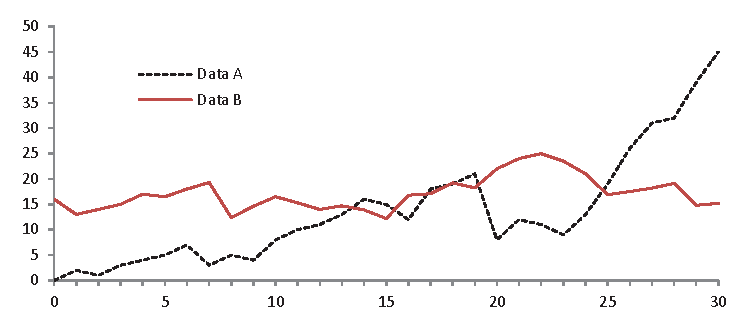
\includegraphics[width=\textwidth]{fig1.eps}
	\caption{Descripción de la figura1.} \label{fig1}
\end{figure}

\begin{table}
	\caption{Descripción de la tabla2}\label{tab2}
\end{table}

\begin{figure}
	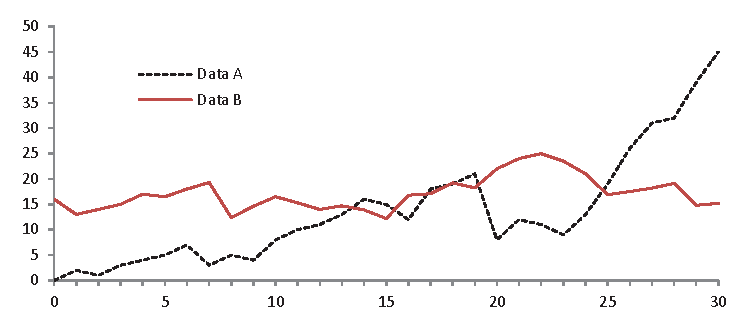
\includegraphics[width=\textwidth]{fig1.eps}
	\caption{Descripción de la figura2.} \label{fig2}
\end{figure}